% Options for packages loaded elsewhere
\PassOptionsToPackage{unicode}{hyperref}
\PassOptionsToPackage{hyphens}{url}
\PassOptionsToPackage{dvipsnames,svgnames,x11names}{xcolor}
%
\documentclass[
  letterpaper,
  DIV=11,
  numbers=noendperiod]{scrartcl}

\usepackage{amsmath,amssymb}
\usepackage{iftex}
\ifPDFTeX
  \usepackage[T1]{fontenc}
  \usepackage[utf8]{inputenc}
  \usepackage{textcomp} % provide euro and other symbols
\else % if luatex or xetex
  \usepackage{unicode-math}
  \defaultfontfeatures{Scale=MatchLowercase}
  \defaultfontfeatures[\rmfamily]{Ligatures=TeX,Scale=1}
\fi
\usepackage{lmodern}
\ifPDFTeX\else  
    % xetex/luatex font selection
\fi
% Use upquote if available, for straight quotes in verbatim environments
\IfFileExists{upquote.sty}{\usepackage{upquote}}{}
\IfFileExists{microtype.sty}{% use microtype if available
  \usepackage[]{microtype}
  \UseMicrotypeSet[protrusion]{basicmath} % disable protrusion for tt fonts
}{}
\makeatletter
\@ifundefined{KOMAClassName}{% if non-KOMA class
  \IfFileExists{parskip.sty}{%
    \usepackage{parskip}
  }{% else
    \setlength{\parindent}{0pt}
    \setlength{\parskip}{6pt plus 2pt minus 1pt}}
}{% if KOMA class
  \KOMAoptions{parskip=half}}
\makeatother
\usepackage{xcolor}
\setlength{\emergencystretch}{3em} % prevent overfull lines
\setcounter{secnumdepth}{-\maxdimen} % remove section numbering
% Make \paragraph and \subparagraph free-standing
\makeatletter
\ifx\paragraph\undefined\else
  \let\oldparagraph\paragraph
  \renewcommand{\paragraph}{
    \@ifstar
      \xxxParagraphStar
      \xxxParagraphNoStar
  }
  \newcommand{\xxxParagraphStar}[1]{\oldparagraph*{#1}\mbox{}}
  \newcommand{\xxxParagraphNoStar}[1]{\oldparagraph{#1}\mbox{}}
\fi
\ifx\subparagraph\undefined\else
  \let\oldsubparagraph\subparagraph
  \renewcommand{\subparagraph}{
    \@ifstar
      \xxxSubParagraphStar
      \xxxSubParagraphNoStar
  }
  \newcommand{\xxxSubParagraphStar}[1]{\oldsubparagraph*{#1}\mbox{}}
  \newcommand{\xxxSubParagraphNoStar}[1]{\oldsubparagraph{#1}\mbox{}}
\fi
\makeatother


\providecommand{\tightlist}{%
  \setlength{\itemsep}{0pt}\setlength{\parskip}{0pt}}\usepackage{longtable,booktabs,array}
\usepackage{calc} % for calculating minipage widths
% Correct order of tables after \paragraph or \subparagraph
\usepackage{etoolbox}
\makeatletter
\patchcmd\longtable{\par}{\if@noskipsec\mbox{}\fi\par}{}{}
\makeatother
% Allow footnotes in longtable head/foot
\IfFileExists{footnotehyper.sty}{\usepackage{footnotehyper}}{\usepackage{footnote}}
\makesavenoteenv{longtable}
\usepackage{graphicx}
\makeatletter
\def\maxwidth{\ifdim\Gin@nat@width>\linewidth\linewidth\else\Gin@nat@width\fi}
\def\maxheight{\ifdim\Gin@nat@height>\textheight\textheight\else\Gin@nat@height\fi}
\makeatother
% Scale images if necessary, so that they will not overflow the page
% margins by default, and it is still possible to overwrite the defaults
% using explicit options in \includegraphics[width, height, ...]{}
\setkeys{Gin}{width=\maxwidth,height=\maxheight,keepaspectratio}
% Set default figure placement to htbp
\makeatletter
\def\fps@figure{htbp}
\makeatother

\usepackage{booktabs}
\usepackage{longtable}
\usepackage{array}
\usepackage{multirow}
\usepackage{wrapfig}
\usepackage{float}
\usepackage{colortbl}
\usepackage{pdflscape}
\usepackage{tabu}
\usepackage{threeparttable}
\usepackage{threeparttablex}
\usepackage[normalem]{ulem}
\usepackage{makecell}
\usepackage{xcolor}
\KOMAoption{captions}{tableheading}
\usepackage{float}
\floatplacement{table}{H}
\usepackage{booktabs}
\usepackage{caption}
\makeatletter
\@ifpackageloaded{caption}{}{\usepackage{caption}}
\AtBeginDocument{%
\ifdefined\contentsname
  \renewcommand*\contentsname{Table of contents}
\else
  \newcommand\contentsname{Table of contents}
\fi
\ifdefined\listfigurename
  \renewcommand*\listfigurename{List of Figures}
\else
  \newcommand\listfigurename{List of Figures}
\fi
\ifdefined\listtablename
  \renewcommand*\listtablename{List of Tables}
\else
  \newcommand\listtablename{List of Tables}
\fi
\ifdefined\figurename
  \renewcommand*\figurename{Figure}
\else
  \newcommand\figurename{Figure}
\fi
\ifdefined\tablename
  \renewcommand*\tablename{Table}
\else
  \newcommand\tablename{Table}
\fi
}
\@ifpackageloaded{float}{}{\usepackage{float}}
\floatstyle{ruled}
\@ifundefined{c@chapter}{\newfloat{codelisting}{h}{lop}}{\newfloat{codelisting}{h}{lop}[chapter]}
\floatname{codelisting}{Listing}
\newcommand*\listoflistings{\listof{codelisting}{List of Listings}}
\makeatother
\makeatletter
\makeatother
\makeatletter
\@ifpackageloaded{caption}{}{\usepackage{caption}}
\@ifpackageloaded{subcaption}{}{\usepackage{subcaption}}
\makeatother

\ifLuaTeX
  \usepackage{selnolig}  % disable illegal ligatures
\fi
\usepackage{bookmark}

\IfFileExists{xurl.sty}{\usepackage{xurl}}{} % add URL line breaks if available
\urlstyle{same} % disable monospaced font for URLs
\hypersetup{
  pdftitle={Exploring the Impact of Dietary and Environmental Factors on Hypertension and Mercury Exposure},
  pdfauthor={Danish Maknojia, Mona Saeed, Leonard Eshun, Su Zhang},
  colorlinks=true,
  linkcolor={blue},
  filecolor={Maroon},
  citecolor={Blue},
  urlcolor={Blue},
  pdfcreator={LaTeX via pandoc}}


\title{Exploring the Impact of Dietary and Environmental Factors on
Hypertension and Mercury Exposure}
\usepackage{etoolbox}
\makeatletter
\providecommand{\subtitle}[1]{% add subtitle to \maketitle
  \apptocmd{\@title}{\par {\large #1 \par}}{}{}
}
\makeatother
\subtitle{2024-12-14}
\author{Danish Maknojia, Mona Saeed, Leonard Eshun, Su Zhang}
\date{}

\begin{document}
\maketitle


\subsection{Abstract}\label{abstract}

Investigating factors influencing blood pressure and mercury levels in
the US population is crucial for public health interventions and
environmental policy-making. This study aims to examine the
relationships between dietary sodium intake and blood pressure levels,
as well as factors that influence blood mercury levels. The dataset
analyzed is derived from the Center for Disease Control (CDC) survey
data collected through interviews, blood tests, and medical examinations
from August 2021 to August 2023. Multinomial regression was used to
model blood pressure levels, and linear regression was applied to model
blood mercury levels. The analysis revealed no significant association
between dietary sodium consumption and blood pressure levels. However,
age emerged as a significant predictor of hypertension (p \textless{}
0.001). As Age increases, the likelihood of having Stage 2 Hypertension
(versus Normal) increases, holding other factors constant. Tap water
intakes, age, and income level have a significant positive association
with blood mercury level (p \textless{} 0.001). Non-Hispanic Asians have
significantly higher mercury level (149.9\%) compared with reference
group of Mexicans Americans. Females on average have mercury levels 8\%
lower compared to males. Our study identified key water intake and
demographic factors affecting blood mercury levels, which can inform
public health policies regarding water consumption and exposure to
environmental toxins.

\subsection{Introduction}\label{introduction}

Hypertension and environmental exposure to mercury are significant
public health concerns worldwide (National Center for Biotechnology
Information, 2021). With hypertension, affecting over 1.28 billion
adults worldwide with a majority in low- and middle-income countries,
and environmental mercury exposure, linked to cardiovascular and
neurological issues such as elevated blood pressure even at low levels,
are significant global public health concerns (World Health
Organization; Houston, p 621). Understanding the factors that influence
these conditions is critical to improving health outcomes and developing
targeted interventions. This study leverages data from the U.S Centers
for Disease Control and Prevention (CDC), a nationally representative
dataset, to explore two key research questions that address these
pressing health issues.

The first research question examines the association between dietary
sodium intake and blood pressure levels, with a particular focus on
whether the effect varies by factors such as gender and race. Blood
pressure is an ordinal variable, categorized into four levels according
to CDC guidelines, ranging from normal to Stage 2 hypertension (CDC,
2023). High dietary sodium intake has long been implicated as a risk
factor for hypertension, a leading contributor to cardiovascular
diseases globally (World Health Organization, 2021). Gender and race may
further modulate this relationship due to physiological and social
determinants of health, making it essential to explore these
interactions. Answering this question provides insights that can inform
dietary guidelines and public health policies aimed at reducing
hypertension-related morbidity and mortality.

The second research question investigates the impact of drinking water
sources, such as tap or bottled water, on blood mercury levels. Blood
mercury is a continuous variable that reflects exposure to mercury, a
toxic heavy metal with known adverse effects on neurological and
cardiovascular health (Agency for Toxic Substances and Disease Registry,
2023). Factors such as race may influence this relationship, potentially
due to disparities in environmental exposure or differences in water
consumption patterns. This question is vital because understanding the
relationship between water sources and mercury exposure can guide
environmental regulations and public health recommendations,
particularly in vulnerable populations.

These research questions address two critical dimensions of health:
dietary and environmental factors. By exploring the interplay between
dietary sodium, drinking water sources, and key demographic factors,
this study aims to provide actionable insights into mitigating the risks
of hypertension and mercury toxicity. The findings have the potential to
inform individual behavioral changes, public health interventions, and
broader environmental and dietary policies.

\subsection{Methods}\label{methods}

\subsubsection{Data Overview and
Preprocessing}\label{data-overview-and-preprocessing}

The dataset used for the first research question consists of information
on 7,801 observations, including variables such as sodium intake, blood
pressure categories, gender, race, age, and alcohol consumption. The
outcome variable, \textbf{blood pressure category}, is ordinal and
categorized as \emph{Normal}, \emph{Elevated}, \emph{Stage 1
Hypertension}, and \emph{Stage 2 Hypertension} based on both the
systolic and diastolic blood measurements as illustrated in the table
below. There were 1830 observations with missing values for alcohol
consumption and sodium intake and 323 observations have missing values
in systolic and diastolic blood pressure measurements.

\begin{longtable}[]{@{}
  >{\raggedright\arraybackslash}p{(\columnwidth - 4\tabcolsep) * \real{0.3288}}
  >{\raggedright\arraybackslash}p{(\columnwidth - 4\tabcolsep) * \real{0.3288}}
  >{\raggedright\arraybackslash}p{(\columnwidth - 4\tabcolsep) * \real{0.3425}}@{}}
\toprule\noalign{}
\begin{minipage}[b]{\linewidth}\raggedright
Blood Pressure Category
\end{minipage} & \begin{minipage}[b]{\linewidth}\raggedright
Systolic Blood Pressure
\end{minipage} & \begin{minipage}[b]{\linewidth}\raggedright
Diastolic Blood Pressure
\end{minipage} \\
\midrule\noalign{}
\endhead
\bottomrule\noalign{}
\endlastfoot
Normal & \textless120 mmHg & and \textless80 mmHg \\
Elevated & 120-129 mmHg & and \textless80 mmHg \\
Stage 1 Hypertension & 130-139 mmHg & or 80-89 mmHg \\
Stage 2 Hypertension & ≥140 mmHg & or ≥90 mmHg \\
\end{longtable}

The systolic and diastolic blood measurements used in this analysis
represent the mean of the three measurements taken for each participant
in the original dataset. These measurements were taken on three
consecutive days. Predictor variables include continuous variables
(e.g., sodium intake, age, alcohol consumption) and categorical
variables (e.g., gender, race).

For the second research question on blood mercury level, the data has
7785 observations, among which 2870 observations have missing values in
either predictor or outcome variables. This dataset has missing values
in variables of mercury level, income level, and water intakes of
bottled water and tap water.

Stochastic regression imputations were used to handle missing values
because (1) dataset size is large enough to build reliable imputation
models; (2) missing values appear in both predictors and outcome
variables; (3) maintains the natural associations in the data; (4)
better than median or mean imputations, which are more arbitrary and
underestimate variance. Extreme outliers in sodium intake and alcohol
consumption were identified using visualizations (boxplots) and summary
statistics. Sensitivity analyses were planned to evaluate the impact of
including these points. Descriptive statistics (mean, median, range) and
visualizations (histograms and boxplots) were used to summarize
continuous variables. Bar charts and frequency tables were used to
explore the distribution of categorical variables. Relationships between
sodium intake and blood pressure levels were explored using boxplots and
correlation analyses. Associations between other predictors (e.g.,
gender, age, race) and blood pressure categories were examined.

\subsubsection{Model Fitting and
Evaluation}\label{model-fitting-and-evaluation}

To examine the relationships between sodium intake and blood pressure
categories, a multinomial logistic regression model was developed. The
initial model included main effects for sodium intake, age, gender,
race, and alcohol consumption. Interaction terms between sodium intake
and gender, as well as sodium intake and race, were later introduced to
assess whether the effect of sodium intake on blood pressure categories
varied across these demographic subgroups. This allowed for the
evaluation of potential effect modification.

Model comparison was performed using the Akaike Information Criterion
(AIC), which balances goodness of fit with model complexity. By
comparing AIC values for models with and without interaction terms, we
determined whether the improved fit provided by the interaction terms
justified the added complexity. Additionally, a confusion matrix was
used to evaluate the predictive performance of the multinomial logistic
regression model.

For modeling blood mercury levels, a multiple linear regression (MLR)
model was employed. Residual vs.~fitted plots were analyzed to assess
linearity and homoscedasticity, while R-squared was used to evaluate the
model's explanatory power. Variance Inflation Factors (VIFs) were
calculated to detect multicollinearity among predictors, with a
threshold of 10 used to identify variables for potential removal or
transformation.

All statistical analyses and modeling were conducted using the R
programming language. Model fit for both the multinomial and linear
regression models was evaluated using AIC and deviance as key metrics.

\subsection{Results}\label{results}

\subsubsection{Research Question 1: Contributing Factors of Blood
Pressure
Category}\label{research-question-1-contributing-factors-of-blood-pressure-category}

Exploratory data analysis (EDA) revealed several important insights.
First, the sodium intake variable contained outliers with extremely high
values, which could potentially skew the results. To address this, we
limited sodium intake values to a maximum of 15,000 mg. This threshold
was chosen based on the distribution of the data and practical dietary
considerations.

Second, we observed that one of the racial groups had no observations in
the dataset, leading to its exclusion from further analysis.
Consequently, the analysis was restricted to six racial groups to ensure
meaningful and interpretable results.

Third, we noted that the ``Normal'' blood pressure category had the
highest number of observations among all categories. This imbalance
suggests that the multinomial regression model may estimate higher
probabilities for the ``Normal'' category compared to others, reflecting
the underlying distribution of the data. The table below shows the
summary statistics of our continuous variables.

\begin{longtable}[]{@{}
  >{\raggedright\arraybackslash}p{(\columnwidth - 8\tabcolsep) * \real{0.3562}}
  >{\raggedleft\arraybackslash}p{(\columnwidth - 8\tabcolsep) * \real{0.1233}}
  >{\raggedleft\arraybackslash}p{(\columnwidth - 8\tabcolsep) * \real{0.1233}}
  >{\raggedleft\arraybackslash}p{(\columnwidth - 8\tabcolsep) * \real{0.1233}}
  >{\raggedleft\arraybackslash}p{(\columnwidth - 8\tabcolsep) * \real{0.2740}}@{}}
\toprule\noalign{}
\begin{minipage}[b]{\linewidth}\raggedright
Variable Name
\end{minipage} & \begin{minipage}[b]{\linewidth}\raggedleft
Minimum
\end{minipage} & \begin{minipage}[b]{\linewidth}\raggedleft
Maximum
\end{minipage} & \begin{minipage}[b]{\linewidth}\raggedleft
Mean
\end{minipage} & \begin{minipage}[b]{\linewidth}\raggedleft
Standard Deviation
\end{minipage} \\
\midrule\noalign{}
\endhead
\bottomrule\noalign{}
\endlastfoot
Sodium Intake & 0 & 20006 & 3061.72 & 1411.03 \\
Diastolic Blood Pressure & 34 & 139 & 72.21 & 11.24 \\
Systolic Blood Pressure & 71.33 & 232.33 & 119.04 & 17.86 \\
Alcohol Consumption & -0.66 & 448.1 & 6.02 & 17.68 \\
Age & 8 & 80 & 44.83 & 22.72 \\
\end{longtable}

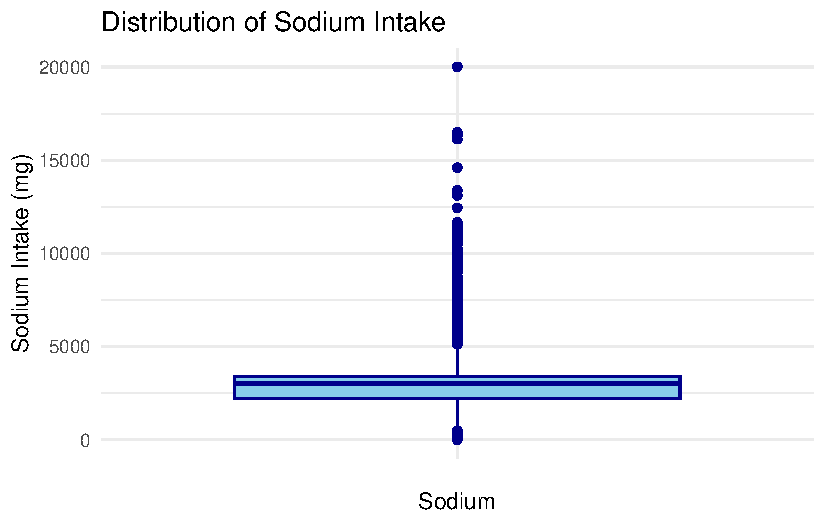
\includegraphics{_IDS702_Final_Report_Feedback_files/figure-pdf/unnamed-chunk-6-1.pdf}

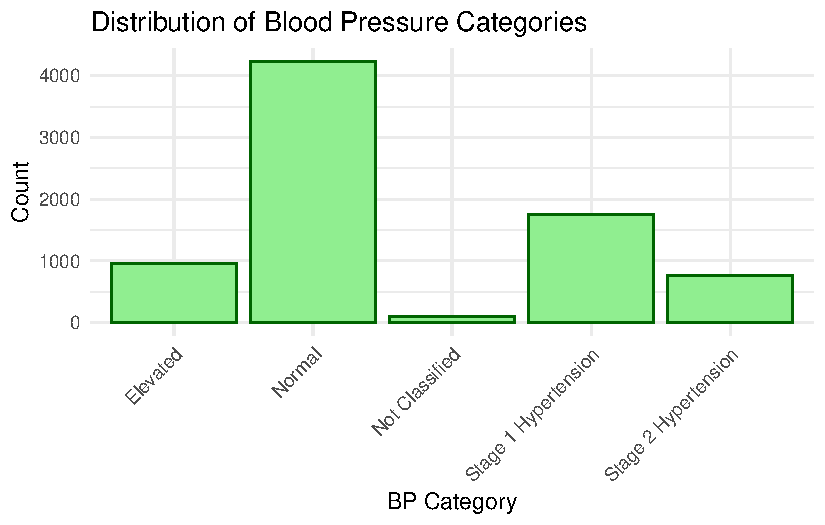
\includegraphics{_IDS702_Final_Report_Feedback_files/figure-pdf/unnamed-chunk-6-2.pdf}

The model's AIC of 12037.52 reflects a balance between complexity and
fit. The confusion matrix shows the highest accuracy in predicting the
``Normal'' category but some misclassifications among hypertensive
stages. The multinomial regression model revealed key associations
between blood pressure categories and predictor variables. For
``Elevated,'' the coefficient for sodium intake is negative (-0.000039),
suggesting that increased sodium intake may be associated with reduced
odds of being in this category compared to ``Normal,'' though the effect
size is very small. For ``Stage 1'' and ``Stage 2 Hypertension,'' the
coefficients are positive but small, indicating a slight increase in the
odds of being in these categories with increased sodium intake. Age and
alcohol consumption were positively associated with higher blood
pressure categories, while gender and race demonstrated significant
variation; for instance, females had lower odds of elevated and
hypertensive categories, and ``Non-Hispanic Black'' was associated with
higher odds of ``Stage 1'' and ``Stage 2 Hypertension.'' Interaction
terms highlighted nuanced relationships, such as weaker sodium intake
effects for females but varying effects across racial groups. Predicted
probabilities provided insights into classification confidence, with age
and alcohol consistently influencing outcomes. While the model converged
successfully, the modest effect sizes for some predictors and potential
for further refinement suggest opportunities for further investigation.

\subsubsection{Research Question 2: Contributing Factors of Blood
Mercury
Level}\label{research-question-2-contributing-factors-of-blood-mercury-level}

Our statistical approach employed multiple linear regression with
log-transformed mercury levels as the dependent variable, addressing
both the non-normal distribution of mercury concentrations and the
presence of detection limits in the measurements. The model incorporated
water consumption variables (tap and bottled water intake), demographic
characteristics (race, gender, age), and socioeconomic status
(income-to-poverty ratio) to capture the complex relationships between
these factors. Below is a summary descriptive statistics of both
dependent variable and priori predictor variables.

\begin{table}[!h]
\centering
\caption{Summary Statistics of Variables}
\centering
\resizebox{\ifdim\width>\linewidth\linewidth\else\width\fi}{!}{
\fontsize{10}{12}\selectfont
\begin{tabular}[t]{l|r|r|r|r}
\hline
Variable & Mean & Standard Deviation & Median & Missing Values\\
\hline
Age & 44.83 & 22.72 & 47.00 & 0\\
\hline
Ratio of Family Income to Poverty & 2.79 & 1.66 & 2.61 & 1000\\
\hline
Tap Water Drank Yesterday (gm) & 732.11 & 1138.27 & 240.00 & 1830\\
\hline
Plain Water Drank Yesterday (gm) & 1248.70 & 1204.79 & 1014.00 & 1830\\
\hline
Bottled Water Drank Yesterday (gm) & 516.60 & 891.93 & 0.00 & 1830\\
\hline
Blood Mercury Level (ug/L) & 1.04 & 1.84 & 0.45 & 672\\
\hline
\end{tabular}}
\end{table}

\begin{table}[!h]
\centering
\caption{Summary Table for Categorical Variables}
\centering
\fontsize{10}{12}\selectfont
\begin{tabular}[t]{llrr}
\toprule
  & Category & Count & Percentage\\
\midrule
Mexican American & Mexican American & 674 & 8.6\\
Other Hispanic & Other Hispanic & 870 & 11.2\\
Non-Hispanic White & Non-Hispanic White & 4256 & 54.6\\
Non-Hispanic Black & Non-Hispanic Black & 1005 & 12.9\\
Non-Hispanic Asian & Non-Hispanic Asian & 453 & 5.8\\
\addlinespace
Other Race & Other Race & 543 & 7.0\\
Male & Male & 3595 & 46.1\\
Female & Female & 4206 & 53.9\\
Tap Water & Tap Water & 2778 & 35.6\\
Bottled Water & Bottled Water & 1969 & 25.2\\
\addlinespace
Both & Both & 498 & 6.4\\
None & None & 2556 & 32.8\\
\bottomrule
\end{tabular}
\end{table}

\paragraph{EDA}\label{eda}

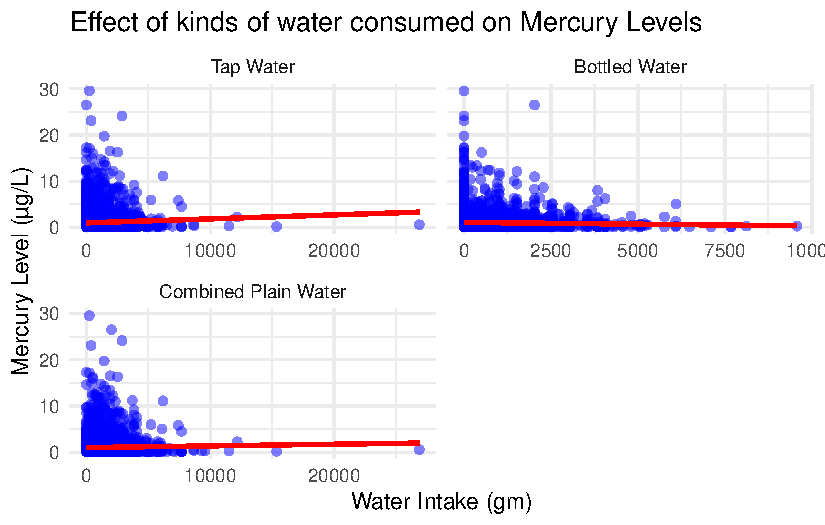
\includegraphics{_IDS702_Final_Report_Feedback_files/figure-pdf/plots-2b-1.pdf}

\begin{enumerate}
\def\labelenumi{\arabic{enumi}.}
\tightlist
\item
  \textbf{Mercury Levels vs.~Water Consumption} The faceted scatter plot
  examined the relationships between mercury levels and water intake
  across three types of water consumption (tap water, bottled water, and
  combined plain water). Linear trend lines showed that higher
  consumption of tap water might led to a slightly increase in blood
  mercury levels in people versus bottled water which had no change in
  blood mercury levels as more is consumed.
\end{enumerate}

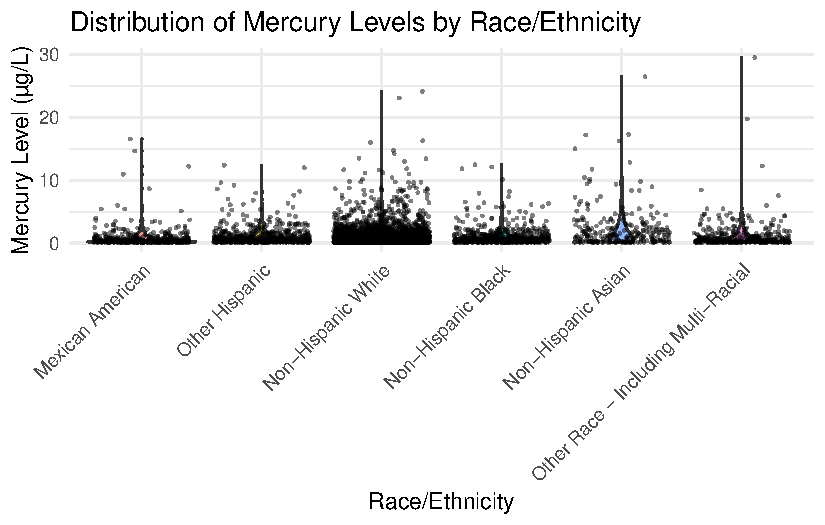
\includegraphics{_IDS702_Final_Report_Feedback_files/figure-pdf/plots-3b-1.pdf}

\begin{enumerate}
\def\labelenumi{\arabic{enumi}.}
\setcounter{enumi}{1}
\tightlist
\item
  \textbf{Mercury Levels by Race/Ethnicity} The violin plot was used to
  compare mercury distributions across racial/ethnic groups. This graph
  shows that mercury levels vary significantly across racial and ethnic
  groups, with Non-Hispanic Asians having the highest levels and the
  widest distribution. We can see that most distribution are
  right-skewed meaning that most individuals in all racial categories
  have low mercury levels, but there are noticeable outliers, especially
  among Non-Hispanic Asians and Non-Hispanic Blacks.
\end{enumerate}

We initially fit a multiple linear regression model towards the blood
mercury levels. However, in the residuals vs fitted graph (in the
appendix section), the spread of residuals increases as the fitted
values grow, indicating heteroscedasticity. The Q-Q plot (in the
appendix section) deviates significantly from the 45-degree reference
line, particularly at the extremes (tails of the distribution),
indicating that the residuals are not normally distributed. These
suggest a potential violation of the normality assumption. Therefore, we
log-transformed the dependent variable to stabilize the variance and
help normalize the residuals.

When fitting the model, we tried to include interaction term between
race and family income to poverty level, because the influence of income
on health outcomes such as mercury levels might vary by race due to
differences in access to healthcare, dietary habits, or exposure to
environmental risk factors and we want to take the heterogeneous effects
into considerations. However, the interaction between race and income
level has a transformed GVIF value of 2.185 (outputs could be found in
appendix), which is slightly high and creates multicollinearity.
Therefore, we decided to remove the interaction term and examine the
effects of race and income level separately.

We also examined the influential points using Cook's distance and marked
the top 5 influential points in below graph. We then refit the model
again after removing these influential points (the model results outputs
and residual plots can be found in appendix section). We also attempted
to remove high leverage points using the threshold of
\(h_i > \frac{2(p+1)}{n}\). However, removing influential points did not
significant change the model results (adjusted R-squared and p-values).
Therefore, we decided to keep these influential points in the model.

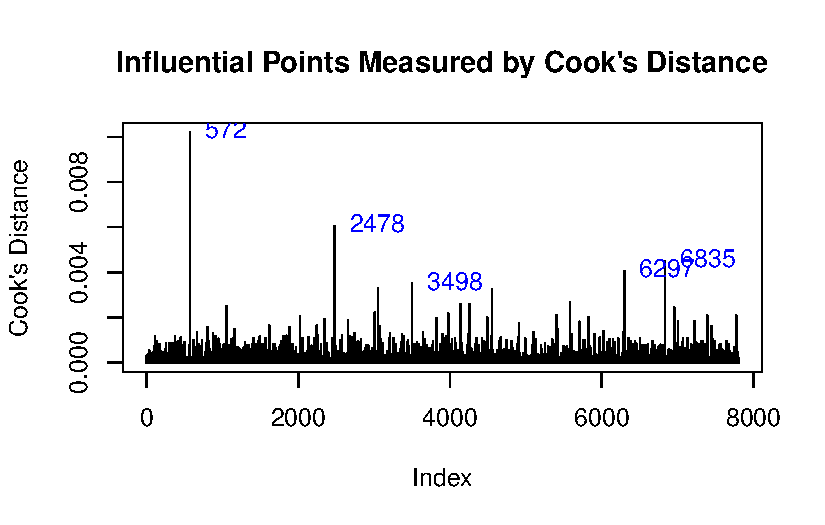
\includegraphics{_IDS702_Final_Report_Feedback_files/figure-pdf/unnamed-chunk-16-1.pdf}

Therefore, the final model was to fit logged blood mercury level using
age, gender, race, income levels, tap water intake and bottle water
intake. The final model outputs are in below table. To make the
coefficients easier to interpret, we performed a back-transformation by
exponentiating the regression coefficients and their confidence
intervals to interpret the results on the original scale of mercury
levels rather than their logged value. This allows us to describe how
each predictor multiplicatively affects mercury levels, providing more
meaningful and practical insights.

The model summary output shows that tap water intakes has a significant
positive association with p-value less than 0.001, whereas bottled water
intake has no significant effect (with p-value of 0.151). For the
variable of race, compared to the reference level of Mexican Americans,
non-Hispanic Asians have 149.9\% higher mercury levels, while
non-Hispanic, non-Hispanic Black and other races have 45\%, 27.4\%,
18.7\% higher mercury levels respectively. The only racial group that
has lower mercury level compared to Mexican Americans is non-Hispanic
White, which estimated to be 9\% lower than the reference group. For
demographic factors, both age and income level have positive association
with mercury levels (with p-value \textless{} 0.001). Holding all other
variables constant, for every unit increase in the income-to-poverty
ratio, mercury levels increase by 14.2\%, which is a bit
counter-intuitive, as the richer family have higher blood mercury level.
Each additional year of age is associated with a 1.4\% increase in
mercury levels. For gender, females, compared to males (the reference
group), have mercury levels that are 8\% lower.

\begin{longtable}[]{@{}lcccc@{}}
\caption{Blood Mercury Levels MLR Model Summary Table (Back-Transformed
Coefficients)}\tabularnewline
\toprule\noalign{}
Predictor Variables & Exp(Beta) & SE & 95\% CI (Exp) & P-value \\
\midrule\noalign{}
\endfirsthead
\toprule\noalign{}
Predictor Variables & Exp(Beta) & SE & 95\% CI (Exp) & P-value \\
\midrule\noalign{}
\endhead
\bottomrule\noalign{}
\endlastfoot
Intercept & 0.160 & 0.058 & 0.143, 0.180 & \textless{} 0.001 \\
Tap Water Intake & 1.000 & 0.000 & 1.000, 1.000 & \textless{} 0.001 \\
Bottled Water Intake & 1.000 & 0.000 & 1.000, 1.000 & 0.151 \\
Race: Other Hispanic & 1.450 & 0.061 & 1.287, 1.634 & \textless{}
0.001 \\
Race: Non-Hispanic White & 0.909 & 0.051 & 0.822, 1.005 & 0.061 \\
Race: Non-Hispanic Black & 1.274 & 0.059 & 1.134, 1.431 & \textless{}
0.001 \\
Race: Non-Hispanic Asian & 2.499 & 0.073 & 2.165, 2.884 & \textless{}
0.001 \\
Race: Other & 1.187 & 0.069 & 1.038, 1.358 & 0.013 \\
Income-to-Poverty Ratio & 1.142 & 0.009 & 1.123, 1.162 & \textless{}
0.001 \\
Gender: Female & 0.920 & 0.027 & 0.873, 0.970 & 0.002 \\
Age (years) & 1.014 & 0.001 & 1.013, 1.015 & \textless{} 0.001 \\
\end{longtable}

The model is statistically significant (F-statistic = 116.8, p
\textless{} 0.001) and explains 12.93\% of the variance in blood mercury
levels with an adjusted R-squared of 0.1293. The model's low R-squared
value is probably because of two possible reasons: (1) There are
outstanding outliers of blood mercury levels, but our model's predictor
variables on demographics and water drinking types are unlikely to be
the key reasons that cause these extremely high mercury levels. The key
reason that could lead to extremely high levels could be environmental
factors, such as serious chemical pollution. (2) For the mercury exam
results, there is lower detection limit. When the actual mercury level
is less than this detection limit of 0.21 µg/L, the value would be
recorded as 0.12 µg/L, which is actual detection limit divided by the
square root of 2. This creates a large cluster of identical values and
true values below detection limit are unknown, which makes it harder for
the model to explain variation that's artificially removed.

We also evaluated the residual plots of the model (plots are in the
appendix section). For the residual plot, there are straight lines in
the middle, which is caused by the detection limit of mercury level. For
the Q-Q plot, the points follow the diagonal line closely, suggesting
good normality in the central part of the distribution. However, there
are some deviations in both tails, which are likely due to the outliers
in the mercury level. VIF analysis is done and there is no
multicollinearity issue in this model.

\subsection{Conclusion}\label{conclusion}

This report sheds light on some of the key factors influencing blood
pressure and mercury levels in the U.S. population. While we didn't find
a significant link between dietary sodium intake and blood pressure, age
stood out as a major predictor of hypertension. This suggests that
efforts to prevent high blood pressure should focus more on age-related
risk factors. When it comes to mercury exposure, tap water consumption,
race, and income emerged as important contributors. Non-Hispanic Asian
populations showed significantly higher mercury levels, which raises
questions about whether dietary factors cause this or if there is
influence from other relationships. To test this we created a model to
determine the strength of factors on mercury levels in individuals. The
complex relationship between race and income also suggests that
environmental exposure risks are not evenly distributed, pointing to
areas where public health policies could make a big difference. Overall,
these findings suggest a more tailored approach to public health---one
that considers individual and community-level differences in exposure
and risk. By combining insights from diet, environment, and
demographics, we can create more effective strategies to reduce
hypertension and mercury toxicity in vulnerable populations.

This study does have some limitations, like the possibility of
confounding variables not included in the model (e.g., physical
activity, environmental factors, genetic predispositions) could
influence blood pressure and blood mercury levels, potentially biasing
the results. Moreover, the reliance on observational data also makes it
harder to draw clear cause-and-effect conclusions. Future research could
consider finding datasets on other relevant variables, such as physical
activity, environmental factors, and genetic markers, to capture a more
comprehensive view of the determinants of blood pressure and mercury
levels. Additionally, identifying thresholds or cutoffs (e.g., sodium or
alcohol intake levels) that have meaningful clinical implications for
blood pressure management would also help increase practical
significance of this statistical analysis. Future research could benefit
from using long-term data and more granular studies to better understand
how individual and environmental factors drive disparities in mercury
exposure and hypertension.

\subsection{References}\label{references}

Centers for Disease Control and Prevention. (2023). High blood pressure
facts and statistics.
\url{https://www.cdc.gov/highbloodpressure/data-research/facts-stats/index.html}

Houston, Michael C. ``The Role of Mercury in Cardiovascular Disease.''
Journal of Clinical Hypertension, vol.~13, no. 8, 2011, pp.~621--627,
https://doi.org/10.1111/j.1751-7176.2011.00489.x.

World Health Organization. ``Hypertension.'' WHO, 2023,
https://www.who.int/news-room/fact-sheets/detail/hypertension.

World Health Organization. (2021). Sodium intake and cardiovascular
health.
\url{https://www.who.int/news-room/fact-sheets/detail/sodium-intake-for-adults-and-children}

Agency for Toxic Substances and Disease Registry. (2023). Mercury and
health. \url{https://www.atsdr.cdc.gov/toxprofiles/tp46.pdf}

National Center for Biotechnology Information. (2021). The clinical
consequences of mercury exposure. PubMed Central. Retrieved from
\url{https://pmc.ncbi.nlm.nih.gov/articles/PMC8108748/}

\subsection{Appendix}\label{appendix}

\paragraph{Research Question 1:}\label{research-question-1}

\subsubsection{Research Question 2:}\label{research-question-2}

\textbf{Residual plots for original model without log transformation}

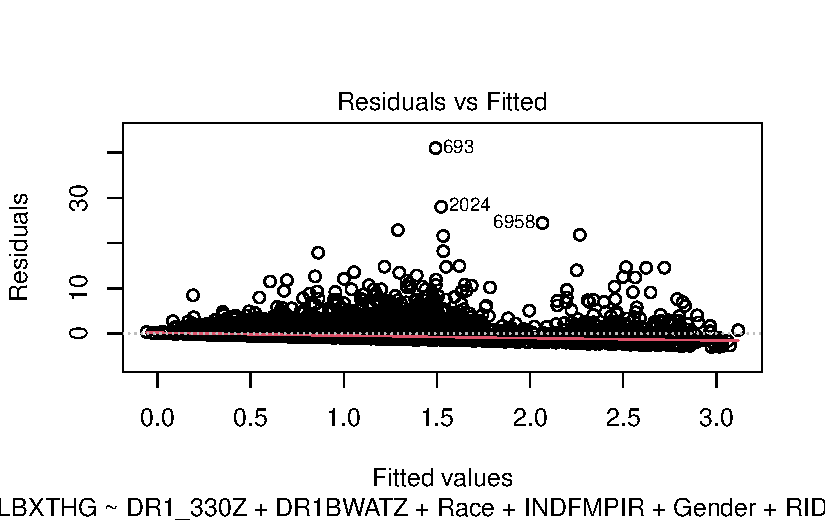
\includegraphics{_IDS702_Final_Report_Feedback_files/figure-pdf/unnamed-chunk-18-1.pdf}

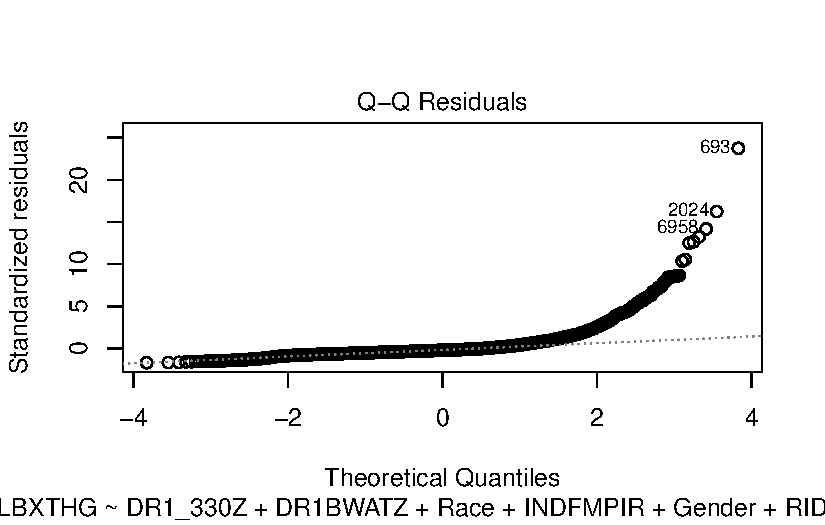
\includegraphics{_IDS702_Final_Report_Feedback_files/figure-pdf/unnamed-chunk-18-2.pdf}

\textbf{Residual plots for finalized model}

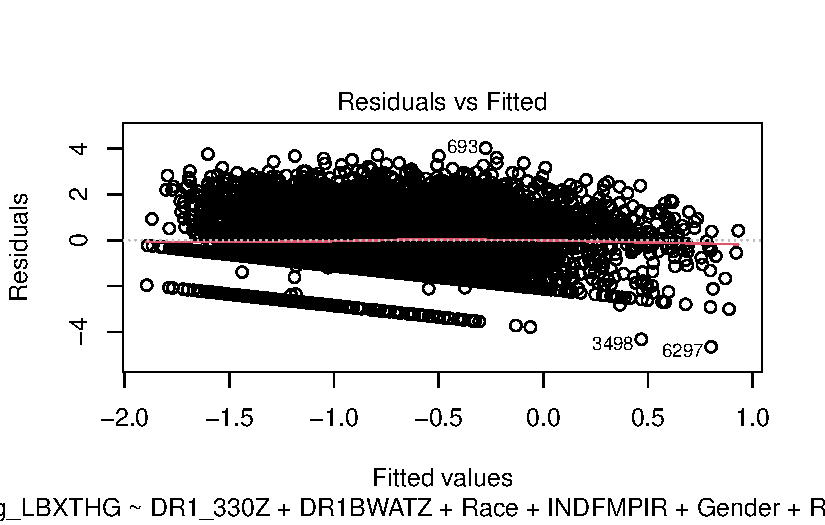
\includegraphics{_IDS702_Final_Report_Feedback_files/figure-pdf/unnamed-chunk-19-1.pdf}

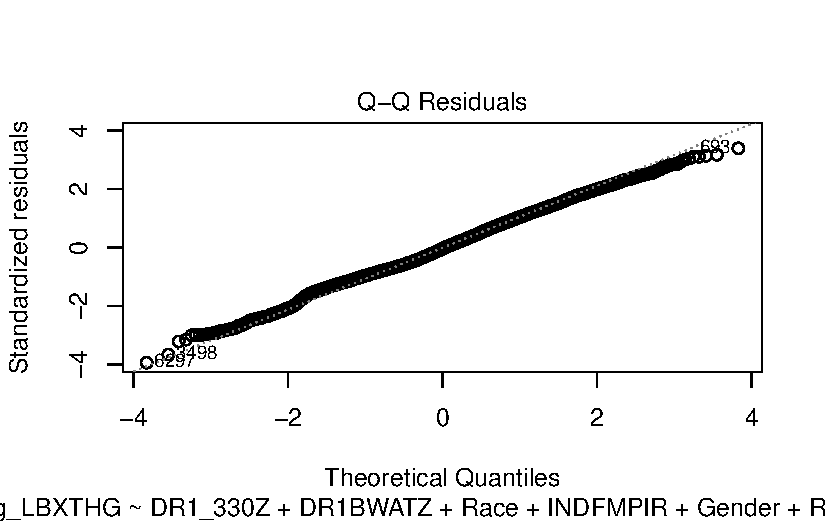
\includegraphics{_IDS702_Final_Report_Feedback_files/figure-pdf/unnamed-chunk-19-2.pdf}

\textbf{VIF analysis of MLR model if include interaction term between
race and income level}

\begin{verbatim}
                     GVIF Df GVIF^(1/(2*Df))
DR1_330Z         1.149411  1        1.072106
DR1BWATZ         1.152138  1        1.073377
Race           462.503174  5        1.847190
INDFMPIR        15.516709  1        3.939125
Gender           1.006728  1        1.003358
RIDAGEYR         1.085340  1        1.041796
Race:INDFMPIR 2477.870494  5        2.184781
\end{verbatim}

\textbf{MLR model results and residual plots after removing top 5
influential points examined through Cook's distance}

\begin{verbatim}

Call:
lm(formula = log_LBXTHG ~ DR1_330Z + DR1BWATZ + Race + INDFMPIR + 
    Gender + RIDAGEYR, data = data_filtered)

Residuals:
    Min      1Q  Median      3Q     Max 
-3.8081 -0.8424 -0.0436  0.8472  4.0322 

Coefficients:
                                          Estimate Std. Error t value Pr(>|t|)
(Intercept)                             -1.844e+00  5.760e-02 -32.005  < 2e-16
DR1_330Z                                 7.535e-05  1.327e-05   5.677 1.42e-08
DR1BWATZ                                 2.975e-05  1.622e-05   1.834   0.0666
RaceOther Hispanic                       3.692e-01  6.077e-02   6.075 1.30e-09
RaceNon-Hispanic White                  -1.007e-01  5.119e-02  -1.967   0.0492
RaceNon-Hispanic Black                   2.435e-01  5.915e-02   4.117 3.89e-05
RaceNon-Hispanic Asian                   9.315e-01  7.308e-02  12.745  < 2e-16
RaceOther Race - Including Multi-Racial  1.687e-01  6.850e-02   2.462   0.0138
INDFMPIR                                 1.339e-01  8.702e-03  15.392  < 2e-16
GenderFemale                            -8.081e-02  2.693e-02  -3.001   0.0027
RIDAGEYR                                 1.397e-02  6.123e-04  22.808  < 2e-16
                                           
(Intercept)                             ***
DR1_330Z                                ***
DR1BWATZ                                .  
RaceOther Hispanic                      ***
RaceNon-Hispanic White                  *  
RaceNon-Hispanic Black                  ***
RaceNon-Hispanic Asian                  ***
RaceOther Race - Including Multi-Racial *  
INDFMPIR                                ***
GenderFemale                            ** 
RIDAGEYR                                ***
---
Signif. codes:  0 '***' 0.001 '**' 0.01 '*' 0.05 '.' 0.1 ' ' 1

Residual standard error: 1.182 on 7785 degrees of freedom
Multiple R-squared:  0.1329,    Adjusted R-squared:  0.1318 
F-statistic: 119.3 on 10 and 7785 DF,  p-value: < 2.2e-16
\end{verbatim}

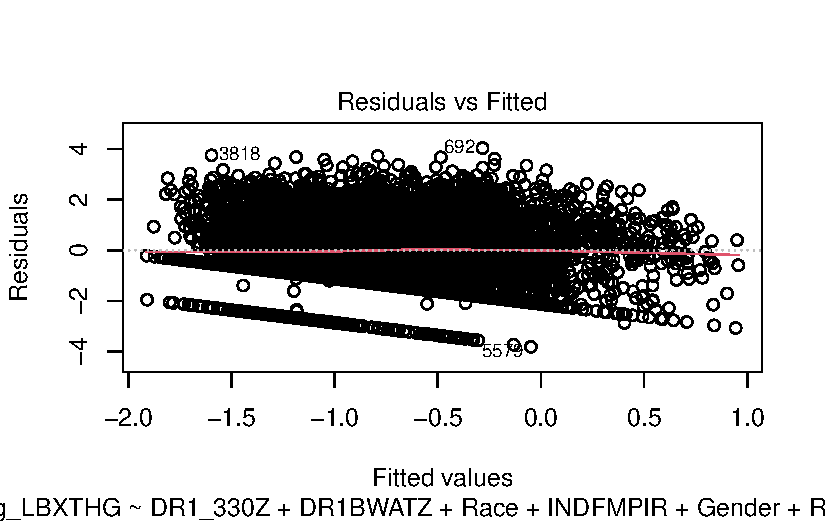
\includegraphics{_IDS702_Final_Report_Feedback_files/figure-pdf/unnamed-chunk-21-1.pdf}

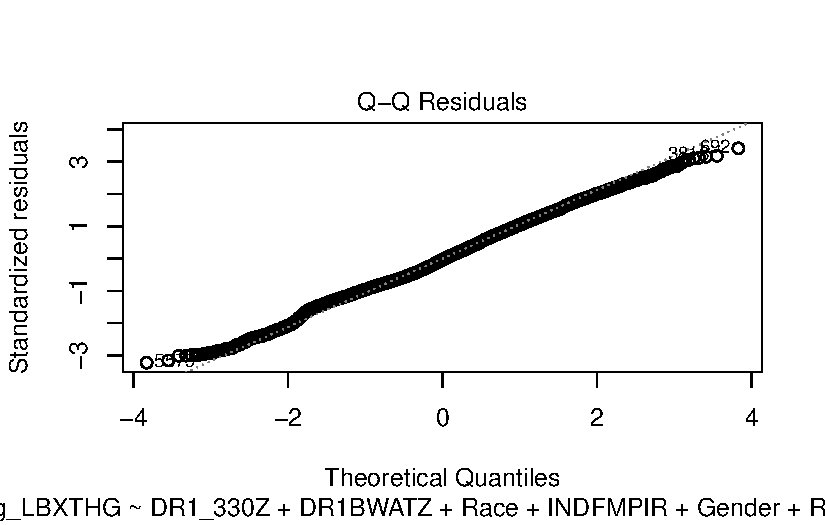
\includegraphics{_IDS702_Final_Report_Feedback_files/figure-pdf/unnamed-chunk-21-2.pdf}

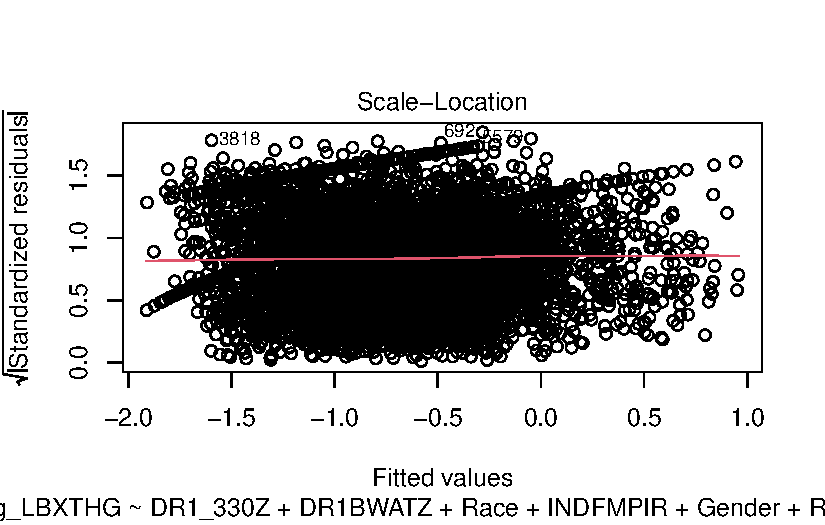
\includegraphics{_IDS702_Final_Report_Feedback_files/figure-pdf/unnamed-chunk-21-3.pdf}

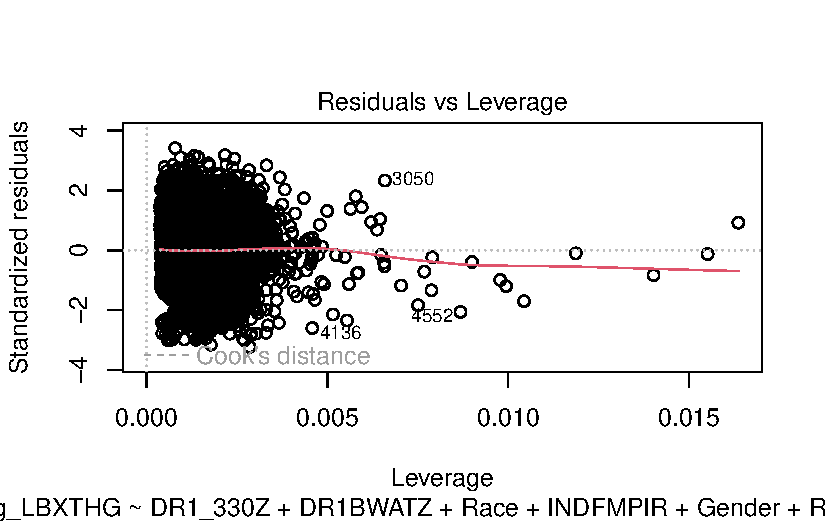
\includegraphics{_IDS702_Final_Report_Feedback_files/figure-pdf/unnamed-chunk-21-4.pdf}

\begin{verbatim}
             GVIF Df GVIF^(1/(2*Df))
DR1_330Z 1.161467  1        1.077714
DR1BWATZ 1.159977  1        1.077022
Race     1.245656  5        1.022209
INDFMPIR 1.176017  1        1.084443
Gender   1.006351  1        1.003171
RIDAGEYR 1.081251  1        1.039832
\end{verbatim}

\textbf{MLR model results and residual plots after removing influential
points higher than high leverage threshold}:

\begin{verbatim}

Call:
lm(formula = log_LBXTHG ~ DR1_330Z + DR1BWATZ + Race + INDFMPIR + 
    Gender + RIDAGEYR, data = data_cleaned)

Residuals:
    Min      1Q  Median      3Q     Max 
-4.5918 -0.8432 -0.0403  0.8422  4.0446 

Coefficients:
                                          Estimate Std. Error t value Pr(>|t|)
(Intercept)                             -1.878e+00  5.860e-02 -32.041  < 2e-16
DR1_330Z                                 9.053e-05  1.497e-05   6.049 1.52e-09
DR1BWATZ                                 4.758e-05  1.859e-05   2.559  0.01051
RaceOther Hispanic                       3.834e-01  6.160e-02   6.223 5.12e-10
RaceNon-Hispanic White                  -8.941e-02  5.205e-02  -1.718  0.08591
RaceNon-Hispanic Black                   2.641e-01  5.991e-02   4.408 1.06e-05
RaceNon-Hispanic Asian                   8.698e-01  7.767e-02  11.198  < 2e-16
RaceOther Race - Including Multi-Racial  1.917e-01  7.008e-02   2.735  0.00625
INDFMPIR                                 1.371e-01  8.892e-03  15.421  < 2e-16
GenderFemale                            -8.611e-02  2.727e-02  -3.158  0.00160
RIDAGEYR                                 1.389e-02  6.206e-04  22.382  < 2e-16
                                           
(Intercept)                             ***
DR1_330Z                                ***
DR1BWATZ                                *  
RaceOther Hispanic                      ***
RaceNon-Hispanic White                  .  
RaceNon-Hispanic Black                  ***
RaceNon-Hispanic Asian                  ***
RaceOther Race - Including Multi-Racial ** 
INDFMPIR                                ***
GenderFemale                            ** 
RIDAGEYR                                ***
---
Signif. codes:  0 '***' 0.001 '**' 0.01 '*' 0.05 '.' 0.1 ' ' 1

Residual standard error: 1.182 on 7603 degrees of freedom
Multiple R-squared:  0.1278,    Adjusted R-squared:  0.1267 
F-statistic: 111.4 on 10 and 7603 DF,  p-value: < 2.2e-16
\end{verbatim}

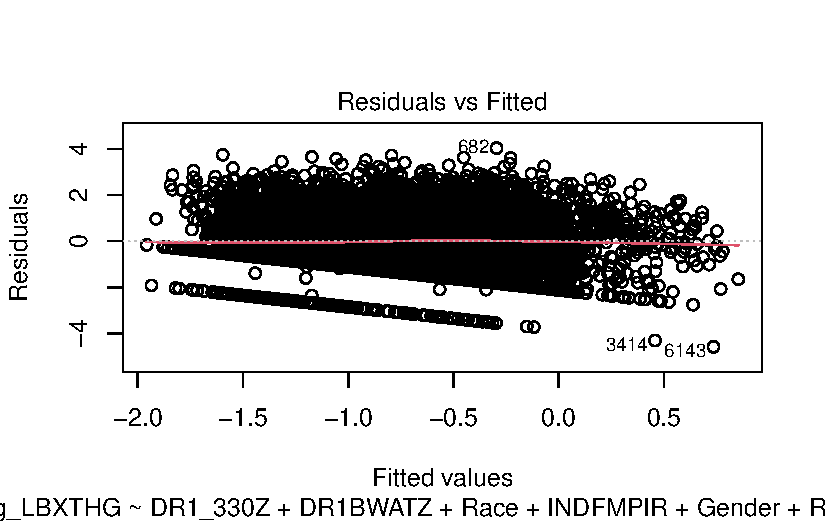
\includegraphics{_IDS702_Final_Report_Feedback_files/figure-pdf/unnamed-chunk-22-1.pdf}

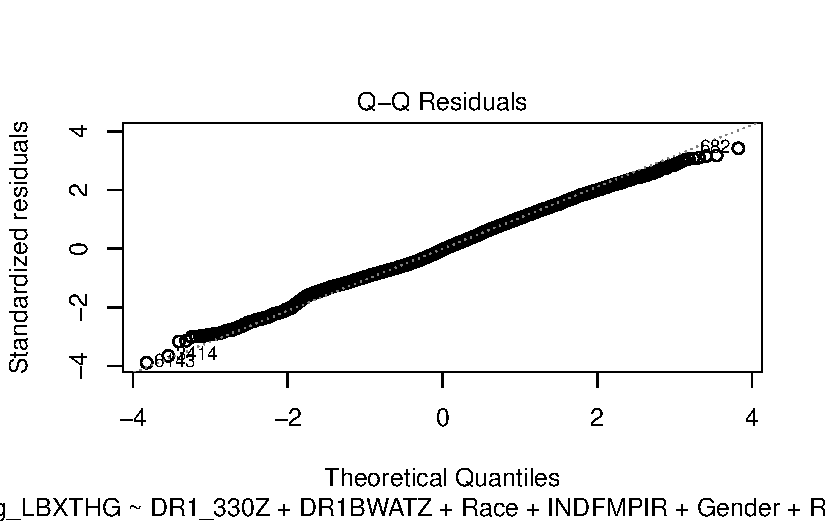
\includegraphics{_IDS702_Final_Report_Feedback_files/figure-pdf/unnamed-chunk-22-2.pdf}

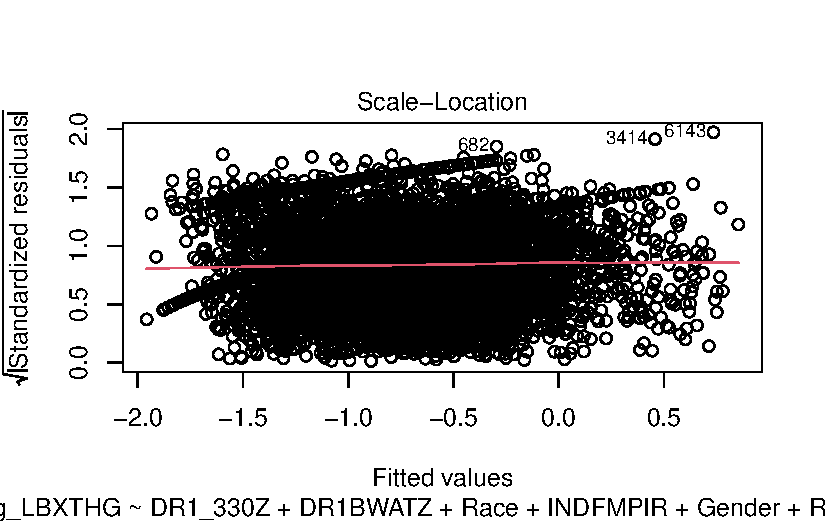
\includegraphics{_IDS702_Final_Report_Feedback_files/figure-pdf/unnamed-chunk-22-3.pdf}

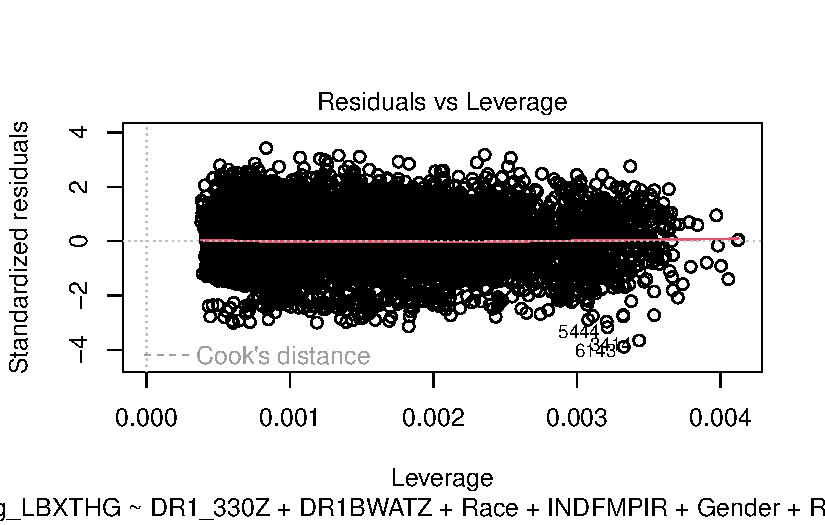
\includegraphics{_IDS702_Final_Report_Feedback_files/figure-pdf/unnamed-chunk-22-4.pdf}

\begin{verbatim}
             GVIF Df GVIF^(1/(2*Df))
DR1_330Z 1.194809  1        1.093073
DR1BWATZ 1.187314  1        1.089640
Race     1.262878  5        1.023614
INDFMPIR 1.188065  1        1.089984
Gender   1.005625  1        1.002809
RIDAGEYR 1.084975  1        1.041621
\end{verbatim}




\end{document}
